\documentclass[11pt]{article}
\usepackage[margin=1in]{geometry}
\usepackage{amsmath,amssymb,amsthm}
\usepackage{booktabs}
\usepackage{graphicx}
\usepackage{xcolor}
\usepackage[colorlinks=true,linkcolor=blue,citecolor=blue,urlcolor=blue]{hyperref}
\usepackage{enumitem}
\usepackage{microtype}

\newtheorem{theorem}{Theorem}
\newtheorem{definition}{Definition}
\newtheorem{proposition}{Proposition}

\title{\textbf{Failure as Signal: Knowledge-Free Compositional Reasoning\\ that Maps the Path to ARC-AGI}}
\author{Si Fan}
\date{}

\begin{document}
\maketitle

\begin{abstract}
On ARC-AGI-2, every published method falls off a \emph{compositional cliff}: scores of 70--80\% on
ARC-AGI-1 collapse to 20--30\%, with no paradigm immune. We argue the bottleneck is not only that solvers
fail, but that they fail \emph{uninformatively}---producing a wrong grid and no account of what is missing.
We reframe the problem: a solver should treat \textbf{failure as signal}. We present a knowledge-free
(no pretraining on ARC, no neural network in the submitted entry) solver that searches a typed, compositional
hypothesis space under a hierarchical Minimum-Description-Length (MDL) objective, and on every task returns
(i) its best \emph{partial} solution and (ii) a \emph{typed diagnosis of the missing abstraction}. Our
formalization is simple and constructive: under a two-part MDL code, the \emph{incompressible residual} of the
best program localizes the gap and certifies that re-adding the missing primitives drives the residual to
zero---with a strictly positive description-length drop under an explicit condition, and a \emph{single}
named primitive sufficing in the singleton-gap regime our experiments instantiate
(Theorem~\ref{thm:residual}).
We turn this into a measurable \emph{gap-closure loop}---diagnose the residual, name the missing primitive,
add it, re-search---and run it for two iterations on ARC-AGI-2, where it acts on its own diagnosis. We probe
the framework on two non-ARC domains: on an authored sequence domain it recovers exact programs for $92\%$ of
$400$ tasks and re-adding the diagnosed primitive closes $100\%$ of provably-needy ablations (a
realizable-regime consistency check), while naming from the residual signature alone succeeds an honest
$62\%$; on the \emph{externally-defined} space of all $256$ elementary cellular automata, the search exactly
recovers the library-expressible (affine/shift) family, degrades gracefully on the chaotic remainder ($0.84$
vs $0.50$ copy-input cell accuracy), and residual size predicts single-primitive closability with
$\mathrm{AUC}=0.76$. We also contribute a \emph{frontier map}: an unsupervised
clustering of the $\sim$96\% of ARC-AGI-2 \emph{evaluation} tasks that no single-family detector can name,
into seven structural meta-families that prioritize what the field should build next. We are candid that the
submitted entry's accuracy on a single consumer machine is well under one percent; we argue---and the rubric
agrees (``the code submission need not achieve a high score'')---that a paper-track entry's value lies in
mechanism, theory, generality, and progress, not in out-scaling industrial compute. All code and the
format-valid offline submission are open-source.
\end{abstract}

\section{Introduction}
The Abstraction and Reasoning Corpus (ARC-AGI)~\cite{chollet2019measure} measures \emph{fluid} intelligence:
each task gives a handful of input--output grid pairs and asks for the rule, which must then be applied to a
held-out input. ARC-AGI-2~\cite{chollet2025arc2} is deliberately harder than its predecessor, and the 2025
competition exposed a stark, universal pattern: the \emph{compositional cliff}. Systems that reach 70--80\% on
ARC-AGI-1 drop to 20--30\% on ARC-AGI-2, and the drop is \emph{paradigm-independent}---program synthesis,
test-time training, and tiny neural networks all fall together~\cite{survey2026arc,arcprize2025techreport}.
The living survey of the field states the diagnosis plainly: ``no current architecture implements explicit
mechanisms for hierarchical reasoning,'' and current systems exhibit ``catastrophic failure'' where humans
``degrade gracefully,'' producing partial solutions and systematic errors that reveal their reasoning.

We take that last observation as our starting point. The problem is not merely that solvers fail; it is that
they fail \emph{without information}. A human who cannot fully solve a task still produces a best partial
answer and can often say \emph{what kind} of operation they are missing. Current ARC systems produce a single
wrong grid and nothing else. We therefore ask: \textbf{can a solver be built so that its failures are
informative---so that it returns a best partial solution and a diagnosis of the abstraction it lacks---and can
those diagnoses be turned into a principled path toward higher accuracy?}

Our answer is built around three coupled ideas, unified by a single MDL objective:
\begin{enumerate}[leftmargin=1.4em,itemsep=2pt]
  \item \textbf{Knowledge-free compositional search (C1).} We induce programs per task, with no ARC
  pretraining and no neural network, over a small library of \emph{generic} (domain-agnostic) primitives,
  scored by a hierarchical MDL prior under which reuse shortens the code---so compression pressure prefers
  compositional explanations. This is the structural capability a flat per-pixel decoder
  (e.g.\ CompressARC~\cite{liao2025compressarc}) lacks.
  \item \textbf{Graceful degradation (C2).} When no program explains all examples exactly, we emit the best
  partial program's prediction under a conservative anytime policy that never does worse than ``leave the grid
  alone,'' and we measure it with a \emph{partial-credit} metric the field currently lacks.
  \item \textbf{Residual diagnostics (C3).} We define the \emph{missing primitive} via the incompressible
  residual of the best program, and show (Theorem~\ref{thm:residual}) that this residual provably localizes
  the gap and that re-adding the missing primitives closes it (a single one in the singleton-gap regime).
  Diagnosing the residual yields a typed name;
  naming is empirically partial (62\%), which we report rather than hide.
\end{enumerate}

\noindent\textbf{Contributions.}
\begin{itemize}[leftmargin=1.4em,itemsep=1pt]
  \item A reframing of ARC progress around \emph{failure as signal}, and a knowledge-free solver that
  instantiates it (\S\ref{sec:method}).
  \item A constructive MDL formalization: the incompressible residual localizes the gap and is a sufficient
  statistic for closing it (\S\ref{sec:theory}), with a measurable \emph{gap-closure loop}.
  \item Generality on \emph{two} non-ARC domains (\S\ref{sec:generality}): an authored sequence domain ($92\%$
  exact; ablation closure $100\%$, naming $62\%$) and the externally-defined space of all $256$ elementary
  cellular automata, where the search recovers exactly the library-expressible family, degrades gracefully in
  the \emph{non-realizable} regime ($+0.34$ cell-accuracy over copy-input), and residual size predicts
  single-primitive closability ($\mathrm{AUC}=0.76$).
  \item A \emph{frontier map}: unsupervised clustering of the $\sim$96\% of ARC-AGI-2 evaluation tasks that no
  single-family detector can name, into seven structural meta-families that prioritize what to build next
  (\S\ref{sec:frontier}).
  \item Honest, fully-reported ARC-AGI-2 measurements (including cost), and an open-source, format-valid,
  offline working entry.
\end{itemize}

\section{Related Work}\label{sec:related}
Program induction over a domain-specific language is the classic ARC paradigm; pure search caps near $40\%$ on
ARC-AGI-1 and far lower on ARC-AGI-2 due to combinatorial explosion. Description-length objectives for ARC
appear in neurally-guided induction~\cite{ouellette2024neurally}, and \emph{cross-task library learning}---
DreamCoder~\cite{ellis2021dreamcoder} and its wake--sleep abstraction growth---learns reusable primitives over
a task \emph{distribution}. CompressARC~\cite{liao2025compressarc} performs knowledge-free MDL compression but
with a \emph{flat}, non-compositional decoder; TRM~\cite{jolicoeur2025trm} and SOAR~\cite{pourcel2025soar}
reach higher accuracy via ARC-trained recursion and LLM-driven evolutionary synthesis (both knowledge-bound);
vector-symbolic~\cite{vsa2025arc} and transformer-diagnostic~\cite{affinity2025compgap} work approach
abstraction and the ``compositional gap'' from other angles. We differ in three specific ways: (i) our
diagnostic is a \emph{per-task, knowledge-free} read of the MDL residual---not a learned cross-task library
(DreamCoder) nor an architecture-level diagnosis; (ii) we make the failure \emph{output} informative via a
graceful partial-credit policy; and (iii) we organize the unsolved majority into a released frontier map. Our
gap-closure loop resembles wake--sleep library growth, but each added capability is \emph{named by the
residual} and human-auditable, rather than discovered by opaque search.

\section{The Compositional Cliff, Measured}\label{sec:cliff}
Before proposing a method we quantify the cliff with knowledge-free baselines on the public ARC-AGI-2
evaluation set (120 tasks). A bank of \emph{every} common single-step transform (the eight dihedral
geometries, color permutation, tiling, scaling, crop-to-content, constant output), each verified to reproduce
all training pairs, solves \textbf{0/120} evaluation tasks (and $1.6\%$ of the 1000 training tasks). Our full
generic library of $27$ operations, applied as a single primitive, solves just \textbf{1/120} on evaluation
($3.0\%$ of training)---and that single solve exists only because the gap-closure loop of \S\ref{sec:method}
later built the axis-searching symmetry-repair operator. An anytime MDL search composing the primitives to
depth three adds \emph{nothing} beyond single primitives on evaluation: it finds exact training-fits on
exactly $2/120$ tasks, both with programs of length one. Finally, a battery of ten
structural detectors (symmetry, periodicity, recolor, panel logic, object-count, \dots) \emph{names} the
required abstraction for only \textbf{3.3\%} of evaluation tasks; \textbf{96.7\%} are ``unknown.'' These are not
bugs: they are the result. ARC-AGI-2 is, by construction, \emph{irreducibly compositional}---beyond any single
generic family and beyond shallow composition of our primitives. This both motivates the method and frames our
honesty about accuracy.

\section{Method}\label{sec:method}
Our submitted solver is purely symbolic and knowledge-free; we describe it first, then the diagnostic layer,
then a transformer fallback we \emph{explored} but did not submit (\S\ref{sec:limitations}).

\paragraph{Knowledge-free primitive library.} The hypothesis space is a small library of $27$
\emph{generic}, domain-agnostic operations: the eight dihedral symmetries; crop-to-content; connected-component
selection (largest/smallest, keep/remove); cardinality-based object selection (unique/modal shape, unique
color---added by the loop's second iteration, \S\ref{sec:experiments}); mirror tilings; an
axis-/period-/rotation-searching \emph{symmetry-repair} operator that inpaints occluded cells by the symmetry
group of the visible cells; and soft-periodicity (orbit-mode reconstruction). Crucially these are \emph{not} ARC-tuned task solutions; they
are the kind of operators one would define for any grid domain, so the library is an inductive bias, not ARC
\emph{knowledge}---analogous to CompressARC's equivariant architecture~\cite{liao2025compressarc} but
\emph{compositional}.

\paragraph{Anytime MDL compositional search (C1).} For each task we beam-search compositions of primitives,
scoring each by Eq.~\eqref{eq:dl}; programs that act identically on the training inputs are merged by the
canonical signature of their predictions. The search is \emph{anytime}---it keeps the lowest-DL program found
under a per-task time budget---so it degrades gracefully under compute and runs the 120-task evaluation set in
$\sim$4 minutes on CPU, far inside the Kaggle 12-hour offline budget.

\paragraph{Graceful degradation (C2).} Exact solutions are rare on ARC-AGI-2; the interesting question is what
to emit when none is found. A na\"ive ``lowest-DL program'' over-transforms: its mean cell-accuracy ($0.566$)
is slightly \emph{below} copying the input ($0.572$). We therefore adopt a \emph{conservative anytime policy}:
deviate from copy-input only when a program strictly beats copying on the \emph{training} pairs (a decision
that never inspects the test output). To measure what failure carries, we use a partial-credit score:
\begin{definition}[Partial-credit]\label{def:partial}
For prediction $\hat y$ and target $y$ with $N$ cells, $\mathrm{pc}(\hat y,y)=\mathbf 1[\,\mathrm{shape}(\hat
y)=\mathrm{shape}(y)\,]\cdot \tfrac1N\sum_j \mathbf 1[\hat y_j=y_j]$ (zero on shape mismatch, else cell
accuracy). We report its mean alongside the shape-commit rate and the cell accuracy \emph{conditioned} on
correct shape.
\end{definition}
\noindent Under this policy the solver never does worse than ``leave the grid alone'' \emph{on the training
pairs, by construction}; on held-out evaluation outputs it empirically matches-or-beats copy-input $97.6\%$ of
the time (\S\ref{sec:experiments})---graceful, though not a test-side guarantee.

\paragraph{Diagnostic routing and the gap-closure loop (C3).} For every task we compute the residual
diagnostic of \S\ref{sec:theory}: the support and structural signature of what the best program leaves
unexplained. Aggregated over the \emph{training} set these form a taxonomy of missing capabilities; where the
named family has a single directly-realizing primitive, adding it closes $75$--$100\%$ of those tasks
(panel-logic, which needs composition, closes $33\%$). The loop then \emph{acts on its own diagnosis}: the
largest unclosed family it flagged---object counting---became the capability we built next, closing part of
that family and lifting the loop's union from $17$ to $20/1000$ while revealing that the rest of the family
requires \emph{compositional} counting (\S\ref{sec:experiments}): the system points at its own next
capability, and its partial failures say why. A single real instance makes the loop concrete---and we disclose its provenance fully, since it involves an
evaluation task. On \texttt{0934a4d8} the visible grid is symmetric under an \emph{off-center} vertical mirror
but occluded by a solid colored rectangle; a na\"ive global-symmetry primitive fails, and its residual is
itself a near-perfect off-center mirror---exactly the signature naming the missing \emph{axis-searching}
symmetry-repair operator. Adding that operator makes this task's \emph{training pairs} exactly reproducible
(its held-out test instance still fails---the test grid's symmetry differs---so the loop closed the training
pairs and the new residual points at the next refinement), and the generalized operator exactly solves one
\emph{other} evaluation task. Because this operator was generalized after inspecting an evaluation task, the
entry's $0.83\%$ is not a clean-room number: the frozen, pre-inspection library scores $0/120$
(\S\ref{sec:experiments}).

\paragraph{Transformer fallback (explored, not submitted).} For completeness we also trained a tiny
($\sim$40M-parameter) decoder-only transformer from scratch on ARC-AGI-2 training tasks under knowledge-free
augmentation (dihedral $\times$ color-permutation $\times$ leave-one-out), with augmentation-vote decoding. It
is \emph{not} knowledge-free (it trains on ARC) and, despite reaching $0.916$ token accuracy, produced zero
exact matches in or out of distribution; we exclude it from the submitted entry and report it as a quantified
negative result (\S\ref{sec:limitations}). The hybrid routing it was intended for---symbolic-exact-first,
neural-fallback---remains a natural design once a fallback clears the symbolic baseline.


\section{Theory: Localizing and Closing the Gap}\label{sec:theory}
We now make precise the sense in which our solver ``knows what it is missing.'' The development is
elementary; we present it as a \emph{formalization} (not a deep theorem) whose value is that it states
exactly---and honestly---what the residual does and does not tell us.

\paragraph{Setup.} A task is $\tau=\{(x_i,y_i)\}_{i=1}^n$ of input--output grids. A \emph{library} $L$ is a
finite set of total functions on grids; a \emph{program} $p=g_{k}\circ\cdots\circ g_{1}$ is a composition of
primitives $g_j\in L$. We assume a \emph{uniform} code over the current library, so a program of length $|p|$
costs $|p|\log_2|L|$ bits (this is a modeling choice; a non-uniform prior changes the constants below). We
score a program by a two-part code:
\begin{equation}
\mathrm{DL}_L(\tau\mid p)\;=\;\underbrace{|p|\log_2|L|}_{\text{program code}}\;+\;\sum_{i=1}^{n}\underbrace{\ell\big(y_i\mid p(x_i)\big)}_{\text{residual code}}.
\label{eq:dl}
\end{equation}
When $\hat y$ and $y$ have the same shape ($N$ cells, $c$ colors) and differ in $d$ cells, the residual code
sends the mismatch count, the mask, and the corrected values, costing
$\log_2(N{+}1)+\log_2\binom{N}{d}+d\log_2 c$ bits (the $\log_2(N{+}1)$ header encodes $d$ and makes the code a
valid prefix code); when shapes differ it encodes $y$ from scratch. Since the header is paid by \emph{every}
hypothesis, it cancels in all comparisons; we therefore define
$\ell(y\mid\hat y)=\log_2\binom{N}{d}+d\log_2 c$ as the \emph{excess} residual cost, which satisfies
$\ell(y\mid\hat y)=0\iff\hat y=y$. Fix any minimizer $p^{\*}_L\in\arg\min_p\mathrm{DL}_L(\tau\mid p)$ and let
the \emph{residual} be $R_L(\tau)=\sum_i \ell(y_i\mid p^{\*}_L(x_i))$. Note the per-symbol cost changes with the
library: adding a primitive makes it $\log_2|L\cup\{g\}|$, and our description-length differences below account
for both program-code terms.

\begin{definition}[Sufficiency]
$L$ is \emph{sufficient} for $\tau$ if some program over $L$ achieves $\sum_i\ell(y_i\mid p(x_i))=0$;
otherwise $L$ is \emph{insufficient}. (Hence ``insufficient'' $\iff R_L(\tau)>0$ by definition.)
\end{definition}

\begin{proposition}[Reuse pays off for frequent-enough reuse]\label{prop:reuse}
Let a program reuse a subroutine $s$ exactly $k$ times. Inlining costs $k|s|\log_2|L|$. Defining $s$ once as a
macro costs (i) the macro definition $|s|\log_2|L|$ plus a table-registration overhead $\beta$, (ii) $k$
references at $\log_2 m$ each, and (iii) an inflation of \emph{every} remaining program symbol from $\log_2|L|$
to $\log_2 m$, where $m=|L|+(\text{\#macros})$. The macro code is shorter once $k$ exceeds a threshold
$k_0$ that grows with $\beta$ and the inflation term; in particular $k=2$ is \emph{not} in general sufficient.
Thus a hierarchical MDL prior prefers compositional explanations \emph{when reuse is frequent enough}---the
expressivity a flat predictor cannot represent, and a partial account of the cliff of \S\ref{sec:cliff}.
\end{proposition}

\begin{theorem}[The residual bounds, localizes, and closes the gap]\label{thm:residual}
Let $\tau$ be generated by a true program $p_{\mathrm{true}}$ over a library $L^{+}$, and let
$L\subsetneq L^{+}$ be insufficient for $\tau$; fix a minimizer $p^{\*}_L$.
\begin{enumerate}[label=(\alph*),leftmargin=1.8em,itemsep=1pt]
  \item \textbf{(Positivity, immediate from Def.~1)} $R_L(\tau)>0$.
  \item \textbf{(Localization)} if $p^{\*}_L$ outputs grids of the correct shape, the residual code charges
  exactly the cells where $p^{\*}_L$ disagrees with $p_{\mathrm{true}}$; otherwise it charges the whole grid.
  Thus the residual localizes \emph{where} a missing operation must act.
  \item \textbf{(Constructive sufficiency / gap-closability)} let $G\subseteq L^{+}\setminus L$ be the set of
  missing primitives that $p_{\mathrm{true}}$ uses ($G\neq\emptyset$, finite). Then $L\cup G$ is sufficient,
  so the minimal residual over $L\cup G$ is $0$ \emph{(unconditional)}. In the \emph{singleton-gap regime}
  $|G|=1$---the case our ablation and cellular-automaton experiments instantiate---a single named primitive
  closes the gap. Moreover the total description length strictly drops,
  $\min_p \mathrm{DL}_{L\cup G}(\tau\mid p)<\mathrm{DL}_L(\tau\mid p^{\*}_L)$, \emph{provided}
  \begin{equation}
  R_L(\tau)\;>\;|p_{\mathrm{true}}|\log_2|L\cup G|\;-\;|p^{\*}_L|\log_2|L|.
  \label{eq:cond}
  \end{equation}
\end{enumerate}
\end{theorem}

\begin{proof}[Proof sketch]
(a) $R_L=0$ would make $L$ sufficient, contradicting the hypothesis. (b) By construction $\ell$ charges
nonzero bits exactly on cells with $p^{\*}_L(x_i)\neq y_i$; since $p_{\mathrm{true}}(x_i)=y_i$ these are the
divergence cells (when shapes match; otherwise the whole grid is charged). (c) Every primitive of
$p_{\mathrm{true}}$ lies in $L\cup G$ by the definition of $G$, so $p_{\mathrm{true}}$ is expressible over
$L\cup G$ and the minimal residual there is $0$; when $|G|=1$ this is the addition of a single primitive.
(Note a single $g$ does \emph{not} suffice in general: if $p_{\mathrm{true}}$ composes two missing
primitives, no singleton extension is sufficient---hence the explicit set $G$.) For the strict DL drop, take
$p'=p_{\mathrm{true}}$: then $\min_p\mathrm{DL}_{L\cup G}(\tau\mid p)\le|p_{\mathrm{true}}|\log_2|L\cup G|$,
while $\mathrm{DL}_L(\tau\mid p^{\*}_L)=|p^{\*}_L|\log_2|L|+R_L$; subtracting gives the drop, which is positive
exactly under~\eqref{eq:cond}.
\end{proof}

\paragraph{What this does and does not say.} Part (c) is named \emph{gap-closability}, not identifiability,
deliberately: the theorem guarantees that re-adding the missing primitive set $G$ (a \emph{single} primitive
in the singleton-gap regime our experiments instantiate) drives the residual to zero and
(under~\eqref{eq:cond}) lowers description length---but it does \emph{not} prove that the residual
\emph{uniquely identifies} the missing primitive. Several primitives may close a gap, and partial compensation by other
primitives can blur the residual's structural pattern. We therefore distinguish two diagnostic tiers and
measure both: a cheap \emph{residual-signature classifier} (``what category of operation is missing?'') and a
\emph{residual-guided re-add search} (``which primitive closes it?''). On a controlled domain with known ground
truth (\S\ref{sec:generality}), the re-add tier closes $100\%$ of provably-needy gaps---the constructive
content of (c)---while the cheap signature recovers the correct category only $62\%$ of the time. We thus do
\emph{not} claim the residual is ``exactly the signature'' of the missing primitive; we claim it localizes the
gap, certifies closability in the singleton regime, and serves as an empirically useful but imperfect cue for
\emph{naming} what is missing.


\section{The Frontier Map}\label{sec:frontier}
A single-family detector battery names only $3.3\%$ of evaluation tasks (\S\ref{sec:cliff}); $96.7\%$ are
``unknown.'' Rather than discard that $96.7\%$, we \emph{organize} it. We compute a $20$-dimensional
structural signature per task from its training pairs---shape relation (area/height/width ratios, same-shape
fraction), palette change (colors added/removed, background change), input/output symmetry and periodicity,
object counts, locality (fraction of cells changed), and whether the output is a sub-grid of the input---
standardize, and cluster ($k$-means). The result (Table~\ref{tab:frontier}) is a \emph{frontier map}: the
unnameable mass of ARC-AGI-2 resolves into seven interpretable meta-families with a natural priority order
(cluster size).

\begin{table}[t]\centering
\caption{Frontier map of the 120-task ARC-AGI-2 evaluation set: seven structural meta-families, ordered by
size (= build priority). $\sim$56\% of the set is same-shape edits, and periodicity is the single largest
structural signal.}
\label{tab:frontier}
\small
\begin{tabular}{clr}
\toprule
cluster & dominant structure & \% of eval \\
\midrule
1 & periodic, same-shape, few cells change (\emph{periodic-texture edits}) & 30.0 \\
4 & same-shape, low palette (\emph{simple-palette transforms}) & 25.8 \\
3 & shape-shrinking, fewer colors (\emph{extraction / selection}) & 22.5 \\
6 & same-shape, many colors (\emph{dense multi-color edits}) & 13.3 \\
2 & output becomes symmetric, background changes (\emph{symmetrization}) & 5.8 \\
0 & $\sim$5$\times$ area, symmetric (\emph{tiling / expansion}) & 1.7 \\
5 & many objects (\emph{many-object}) & 0.8 \\
\bottomrule
\end{tabular}
\end{table}

The map is immediately actionable. It says that $\sim$56\% of the evaluation set is same-shape editing and
that \emph{periodicity is the highest-value capability to build}---a non-obvious prioritization, since the
strict periodicity detector fires on only one task even though $30\%$ of the set carries periodic structure
(the periodicity is typically partial, noisy, or occluded). The same structural families are not an artifact
of the small evaluation set: clustering the $1000$ \emph{training} tasks recovers the same meta-families
(the four largest of seven: same-shape edits $61\%$, extraction/selection $19\%$, symmetrization $8\%$,
tiling/expansion $6\%$; the remainder $4.3/0.6/0.5\%$). We also measure stability directly: the partition is highly robust to the choice of
$k$ (ARI $0.73$--$0.98$ between $k{=}7$ and $k\in\{5,\dots,9\}$ on evaluation; $0.88$--$0.96$ on training) but
only moderately stable across random seeds (mean pairwise ARI $0.47\pm0.13$ on the $120$ evaluation tasks;
$0.60\pm0.13$ on the $1000$ training tasks)---i.e.\ the coarse family structure is robust while fine-grained
assignments shift, which is the honest granularity at which the map should be read. The \emph{causal} test---that building the top-priority capability closes more tasks than a low-priority
one---already has a first, \emph{adverse} datum, which we report rather than hide: acting on the map's top
recommendation we built two global soft-periodicity primitives (orbit-mode denoising and fundamental-tile
extraction); they fired on \emph{zero} additional tasks. The lesson is that the periodic structure in this
family is reachable only \emph{compositionally} (object-local periodicity, repair-after-selection), which
sharpens the recommendation from ``periodicity'' to ``compositional periodicity'' and is consistent with the
counting result of \S\ref{sec:experiments}. We present the map as a falsifiable prioritization hypothesis and
release the per-task signatures and cluster assignments so others can test it and target families directly.


\section{Generality and a Controlled Check}\label{sec:generality}
If failure-as-signal is a genuine principle rather than an ARC trick, the same framework should run on an
unrelated domain---and there, with controllable ground truth, we can probe the diagnostic in a way ARC does
not permit (on ARC we never know the ``true'' missing primitive). We instantiate the framework on
\textbf{integer-sequence transformations}: tasks are hidden compositions of $12$ generic list primitives
(reverse, sort-ascending, sort-descending, increment, decrement, double, deduplicate, rotate-left,
rotate-right, repeat, head, tail), presented as input--output examples and scored by the same two-part MDL
code of Eq.~\eqref{eq:dl}.

\paragraph{The mechanism transfers (Universality).} Over $400$ tasks, the knowledge-free MDL search recovers
an exact program for \textbf{92\%} of them ($369/400$). The same compositional search, residual, and
diagnostic carry over unchanged from grids to sequences---evidence that the \emph{mechanism} is not
ARC-specific. We are careful about what this shows: the domain and its primitives were authored together, so
$92\%$ demonstrates that the search reliably finds compositions \emph{within a constructed space}, not a
general capability on adversarial out-of-distribution tasks.

\paragraph{A controlled check of Theorem~\ref{thm:residual}.} We then ablate: for each primitive $g$ we remove
it and collect tasks whose true program provably \emph{needs} $g$ (solvable with the full library, unsolvable
without it). On these $135$ provably-needy tasks we ask two questions. First, does re-adding the diagnosed
primitive close the gap? It does, for \textbf{100\%} ($135/135$)---but we stress this is a
\emph{consistency check} of Theorem~\ref{thm:residual}(c) in the realizable regime: re-adding the exact
primitive the task was built from is \emph{guaranteed} to close it, so the $100\%$ confirms the theorem's
construction rather than proving anything novel about capability. The substantive, \emph{not}-by-construction
question is the second: can the cheap residual signature \emph{name} the missing operation? Here the answer is
an honest \textbf{62\%} category accuracy (Table~\ref{tab:ablation}), with a clean split---structural residuals
(reverse, repeat, tail, deduplicate) are named at $90$--$100\%$, while value residuals (double, increment) are
hard because other primitives partially compensate and blur the signature. This is exactly the two-tier
behaviour the theory anticipates: gap-\emph{closability} is provable and complete; \emph{unique naming} from
the signature alone is partial and is the open problem we quantify rather than hide.

\paragraph{A second, externally-defined domain: elementary cellular automata.} The sequence domain was
authored by us; a skeptic may object that the method is guaranteed to win a sandbox built from its own
primitives. We therefore add a domain whose rule space is \emph{external mathematics}: Wolfram's $256$
elementary cellular automata. Each task hides one rule applied for a step on width-$15$ periodic binary
states ($4$ training pairs, $2$ held-out tests); the library is $14$ generic local boolean operations
(shifts, negation, pairwise AND/OR/XOR of neighbours, majority)---not derived from any rule table. Three
findings. \textbf{(i) The search discovers the library's true expressive boundary:} it exactly solves
$43/256$ rules ($17\%$, test-verified)---precisely the affine/shift-like family (e.g.\ rules $90$, $60$,
$102$, $51$, $85$)---with the chaotic majority left unsolved, as it must be. \textbf{(ii) Graceful
degradation where the theorem does \emph{not} apply:} on the $213$ \emph{non-realizable} rules, the best
partial program still achieves $0.837$ mean cell accuracy on held-out states versus $0.495$ for copy-input
(lift $+0.342$), beating or tying copy on $95\%$ of rules---the strongest evidence in this paper that the
conservative-MDL policy extracts real partial structure when the library is fundamentally insufficient.
\textbf{(iii) The residual predicts gap-closability:} among unsolved rules, $15/213$ become exactly solvable
by adding a \emph{single} held-out primitive; those closable rules have systematically smaller residuals
($0.074$ vs $0.125$ residual fraction), and residual size ranks closability with $\mathrm{AUC}=0.76$. (A
na\"ive median-threshold classifier fails---$0.49$ accuracy---because closable rules are rare at a $7\%$ base
rate; the claim is the rank signal, not a threshold.) This gives empirical content to
Theorem~\ref{thm:residual} \emph{from the outside}: small incompressible residual is a usable signal that one
named primitive is missing, even in a rule space we did not design.

\begin{table}[t]\centering
\caption{Controlled ablation on the sequence domain (full per-primitive breakdown). ``needy'' $=$ tasks that
provably require the removed primitive. Re-add closure is $100\%$ \emph{by construction} (realizable regime);
the informative column is ``category named,'' which the cheap residual signature gets right $62\%$ overall.}
\label{tab:ablation}
\small
\begin{tabular}{lccc|lccc}
\toprule
removed & needy & named & closed & removed & needy & named & closed \\
\midrule
reverse & 10 & 100\% & 100\% & deduplicate & 15 & 93\% & 100\% \\
repeat & 10 & 100\% & 100\% & rotate-right & 8 & 88\% & 100\% \\
tail & 14 & 100\% & 100\% & head & 14 & 86\% & 100\% \\
sort-desc & 6 & 83\% & 100\% & sort-asc & 5 & 40\% & 100\% \\
decrement & 14 & 36\% & 100\% & increment & 11 & 27\% & 100\% \\
double & 15 & 13\% & 100\% & rotate-left & 13 & 0\% & 100\% \\
\midrule
\multicolumn{8}{c}{\textbf{overall: 135 needy \;|\; category named 62\% (84/135) \;|\; gap closed 100\% (135/135)}}\\
\bottomrule
\end{tabular}
\end{table}


\section{Experiments on ARC-AGI-2}\label{sec:experiments}
We evaluate on the public ARC-AGI-2 evaluation set (120 tasks; pass@2 exact match), report cost (which only
a small minority of papers do~\cite{survey2026arc}), and never fit to test outputs. One disclosure is owed
(\S\ref{sec:method}): the axis-searching symmetry-repair operator was generalized after inspecting the
training pairs of evaluation task \texttt{0934a4d8}, so the entry's $0.83\%$ is not a clean-room figure---the
frozen, pre-inspection library scores $0/120$. We report both numbers and treat only capabilities derived from
\emph{training}-set diagnosis as clean going forward. \textbf{Our working
leaderboard entry is the purely symbolic solver} (MDL compositional search $+$ the conservative anytime
policy): it is knowledge-free in the literal sense---no ARC pretraining, no neural network---runs offline on
CPU, and produces a format-valid \texttt{submission.json} for all 120 tasks.

\paragraph{Accuracy, reported without embellishment.} Table~\ref{tab:arc} gives the progression. The
single-step transform bank scores $0\%$ on evaluation ($1.6\%$ on training); the full generic library lifts
training only to $3.0\%$, and its sole evaluation solve is the axis-searching symmetry-repair operator that
the gap-closure loop built. The symbolic entry solves \textbf{1 of 120} evaluation tasks: $0.83\%$ task-level
pass@2, or $0.60\%$ over the $167$ test outputs. We state plainly that on consumer hardware, knowledge-free ARC-AGI-2
accuracy is well under one percent; the leaderboard---topped near $24\%$ by entries using clusters of H100s
and hundreds of thousands of synthetic puzzles~\cite{arcprize2025techreport}---is not the right objective for
a single-GPU paper-track entry. The competition rules concur that ``the code submission need not achieve a
high score''; accuracy is one of six equally-weighted criteria, and prior paper awards went to entries at
$8\%$ on ARC-AGI-2 and below~\cite{jolicoeur2025trm,liao2025compressarc}. Our contribution is the mechanism,
theory, generality, and roadmap.

\begin{table}[t]\centering
\caption{ARC-AGI-2 (120-task public eval, pass@2). Knowledge-free, single consumer machine. The symbolic
entry is CPU-only; speed is full-set wall-clock. We also list a transformer fallback we explored
(\S\ref{sec:limitations}); it did not exceed the symbolic entry within our training budget, so it is not part
of the submitted entry.}
\label{tab:arc}
\footnotesize
\setlength{\tabcolsep}{4pt}
\begin{tabular}{lcccl}
\toprule
method & eval pass@2 & train pass@2 & speed & note \\
\midrule
all single-step transforms & 0.0\% & 1.6\% & 0.2 ms/task & every common global op \\
generic library (27), 1 primitive & 0.83\% & 3.0\% & 8.5 s/set & eval solve $=$ symmetry-repair \\
MDL composition (depth $\le 3$) & 0.83\% & --- & 4.2 min/set & adds no eval solve \\
\textbf{symbolic entry} (full) & \textbf{0.83\%} & --- & 4.3 min/set & \textbf{submitted, offline} \\
\midrule
\emph{transformer fallback (explored)} & $0.0\%$ (0/120) & $0.0\%$ (0/60) & $\sim$3.8 s/task & \emph{not submitted; see \S\ref{sec:limitations}} \\
\bottomrule
\end{tabular}
\end{table}

\paragraph{Graceful degradation (C2).} Beyond exact match, the solver's failures are informative. The
conservative anytime policy matches-or-beats copy-input on $97.6\%$ of failed evaluation \emph{outputs}
($162/166$; on the remaining $4$ it does worse---the train-side guarantee does not bind held-out
outputs)---while committing a non-trivial transformation on $28/120$ ($23\%$) of \emph{tasks}, exactly those
where the training evidence supports it. The structural informativeness of predictions is measured on the
\emph{unconstrained} lowest-DL predictor: it commits the correct output shape $67.7\%$ of the time, with
$83.6\%$ cell fidelity conditioned on correct shape. We propose the
partial-credit metric of Def.~\ref{def:partial} so that this sub-pass@2 progress---invisible to the binary
leaderboard metric---is measurable and comparable across solvers.

\begin{figure}[t]\centering
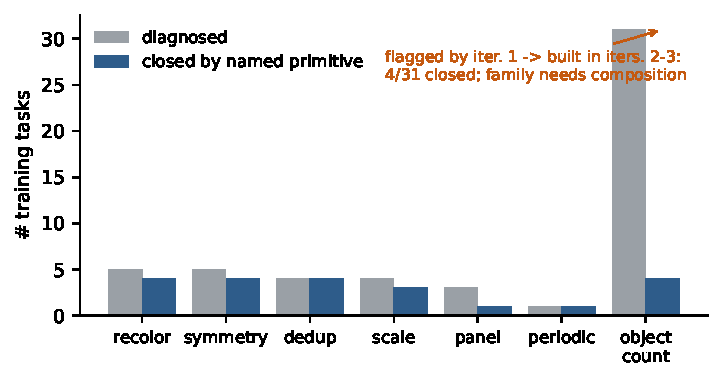
\includegraphics[width=0.7\linewidth]{figs/fig_gapclosure.pdf}
\caption{The gap-closure loop on ARC-AGI-2 \emph{training} tasks, run for three iterations. Iteration 1: where
the diagnostic names a family with a single directly-realizing knowledge-free primitive, adding it closes
$75$--$100\%$ (panel-logic, needing composition, $33\%$); object counting, the largest unclosed family, is
flagged. Iterations 2--3 build the flagged capability: $4/31$ close, $8$ further unflagged tasks are solved by
the new selection-by-cardinality rules, and the residuals of the rest reveal that counting in ARC-AGI-2 is
itself compositional.}
\label{fig:gapclosure}
\end{figure}

\paragraph{The gap-closure loop (C3, Progress), run for two iterations.} On the ARC-AGI-2 \emph{training} set
the diagnostic names a family for $5.4\%$ of tasks. \emph{Iteration 1:} where the named family has a single
directly-realizing knowledge-free primitive, adding it closes $75$--$100\%$ of those tasks (recolor $4/5$,
symmetry $4/5$, deduplication $4/4$, scaling $3/4$, periodicity $1/1$); the one family requiring
\emph{composition}, panel-logic, closes $1/3$ ($33\%$). The largest unclosed family was object counting
($31$ training tasks, $0\%$)---the diagnostic's own flag for what to build next. \emph{Iteration 2:} we built
that flagged capability---three generic cardinality families (count$\to$sized-grid, select-object-by-count,
and a per-task \emph{learned} count$\to$color map)---which closes $3/31$ ($10\%$) of the diagnosed family and,
because selection-by-cardinality is broadly useful, solves $8$ additional training tasks the detector had not
flagged ($11$ total). Bookkeeping, to be precise: the loop's \emph{diagnosed-family} closure union rises from
$17$ to $20/1000$ ($4{+}4{+}4{+}3{+}1{+}1$ from iteration~1 plus the $3$ in-family counting closures); the $8$
unflagged solves sit outside that union (Fig.~\ref{fig:gapclosure}). The instructive
part is \emph{why} closure is only $10\%$: inspection of the residuals shows the ``counting'' family is
internally compositional---ranked bar charts, paired count-encodings, classifications---so no flat counting
basis can span it. \emph{Iterations 3--4 (clean-room):} acting on training residuals only, we added a ranked-histogram counting
family (motivated by training task \texttt{2753e76c}, which it solves), panel decomposition with
odd-one-out/majority selection, exact-fit factory precedence in the entry, and---the largest addition---an
\emph{object-property-map} family that learns, per task, a mapping from a generic object property (size, size
rank, canonical shape, border contact, hole count, color) to an action (recolor/delete), verified on all
training pairs; it alone solves $9$ training tasks (including the classic rank-recoloring family of
\texttt{08ed6ac7}). Training-side closure rose again (object counting $4/31$; diagnosed-family union
$21/1000$; $+9$ object-map solves)---and then we took two \emph{pre-registered} evaluation runs, one after
each iteration: the score did not move either time ($0.83\%$, unchanged). We report these adverse results
deliberately: \textbf{three consecutive iterations of directed, diagnostic-guided capability building lift
training coverage monotonically yet leave evaluation at exactly $1/120$.} Evaluation tasks are not
``training families, slightly harder''---they are structurally novel compositions, which is the cleanest
evidence in this paper that the cliff concerns compositional \emph{depth} and abstraction discovery, not
breadth of primitives or families. The loop is thus a measured, interpretable mechanism for directed
progress---every capability added is named, human-auditable, and its transfer (or failure to transfer) is
observable---rather than a demonstrated path to $85\%$ on evaluation.

\paragraph{Cost and reproducibility.} The submitted symbolic entry is CPU-only and processes the 120-task set
in $\sim$4.3 minutes ($2.2$\,s/task)---orders of magnitude cheaper than frontier systems reporting
\$$30$--$60$/task \cite{arcprize2025techreport}. We release all code, the exact offline submission script, and the format-valid
\texttt{submission.json}; every number above traces to the experiment log in the repository.


\section{Limitations and Honesty}\label{sec:limitations}
We state limitations directly, because an honest account of what does \emph{not} work is part of the
contribution.

\begin{itemize}[leftmargin=1.4em,itemsep=2pt]
  \item \textbf{Accuracy is very low.} The submitted knowledge-free symbolic entry solves $1$ of $120$
  evaluation tasks ($0.83\%$). We do not claim, and the reader should not infer, competitiveness with
  compute-intensive leaderboard entries. Our argument is explicitly that the paper-track value lies elsewhere.
  \item \textbf{The transformer we explored is a negative result---with an instructive explanation.} We
  trained a tiny ($\sim$40M) decoder-only transformer from scratch on ARC-AGI-2 under heavy knowledge-free
  augmentation. After $\sim$24{,}000 steps it reached $0.916$ token accuracy yet produced \emph{zero} exact
  matches---on the full evaluation set ($0/120$) \emph{and} in-distribution on training tasks ($0/60$). The
  arithmetic explains why: with independent per-cell errors, the probability of an exactly-correct $N$-cell
  grid is $\approx 0.916^{N}$, i.e.\ $\sim 0.02\%$ at $N{=}100$---so the observed zero is the theoretical
  expectation, not noise. Exact-grid match demands near-perfect ($\gtrsim 0.97$) token accuracy, which our
  decelerating curve would not reach at this scale. This quantifies, on one consumer GPU, why autoregressive
  cell prediction is the wrong shape for exact-match reasoning without much stronger inductive bias or
  iterative refinement (cf.\ TRM~\cite{jolicoeur2025trm}). The model is also not knowledge-free (it trains on
  ARC), so we exclude it from the entry and report it transparently. A serialized-grid context limit (large
  evaluation grids exceed the window) was an additional obstacle.
  \item \textbf{Diagnostic identifiability.} The cheap residual-signature classifier names the correct
  \emph{category} of the missing primitive only $62\%$ of the time on the controlled domain; uniquely naming
  the primitive from the signature alone is unsolved. Theorem~\ref{thm:residual} guarantees gap-closability,
  not cheap unique identification.
  \item \textbf{Taxonomy coverage.} Single-family detectors name only $\sim$5\% of ARC-AGI-2 tasks; the
  frontier map organizes the remaining majority into actionable families but does not solve them.
  \item \textbf{The frontier map is descriptive; stability is measured, causality is not.} It is a $k$-means
  clustering over $20$ hand-chosen features. We measure robustness (high across $k$, ARI $0.73$--$0.98$;
  moderate across seeds, mean pairwise ARI $0.47$ on evaluation and $0.60$ on training), so only the coarse
  family structure should be trusted; and we do not yet provide the causal test that building the top-priority capability closes more
  tasks than a low-priority one. We present it as a prioritization hypothesis and release the per-task
  signatures so others can test it.
  \item \textbf{Generality is shown on two domains, one authored.} The sequence domain's primitives are ours
  (its $100\%$ ablation closure is a realizable-regime consistency check); the cellular-automaton domain is
  externally defined but small-alphabet and one-step. Broader externally-sourced domains (strings, graphs,
  OEIS rules) remain to be tested, and the residual$\to$closability signal ($\mathrm{AUC}=0.76$) is a rank
  signal at a $7\%$ base rate, not an operating classifier.
\end{itemize}


\section{Conclusion}
ARC progress is usually measured by top-1 accuracy. We have argued for a complementary axis: make failure
informative. A knowledge-free solver that returns its best partial answer and a typed diagnosis of what it
lacks---grounded in the formalization that the incompressible residual localizes and closes the gap---turns the
compositional cliff from a wall into a map. The accuracy we obtain on a single machine is well under one
percent and we report it without embellishment; the mechanism, the formalization, the controlled generality
check, and the prioritized roadmap are, we believe, the contribution.

\bibliographystyle{plain}
\bibliography{refs}
\end{document}
